\documentclass[xcolor={dvipsnames}]{beamer}
\usepackage{amsmath}
% \usepackage{beamerthemesplit} // Activate for custom appearance
\usepackage{hyperref}
\usepackage{ragged2e}

\title{Logistic Regression\\ and the ROC curve}
\author{Schwartz}
\date{\today}

\begin{document}

\frame{\titlepage}

{
\beamertemplatenavigationsymbolsempty

\frame
{
 \frametitle{Odd, even at best}

{
\fontfamily{<familyname>}\selectfont
\begin{quote}
\scriptsize
\justify
%In the 2015/16 season,   incredibly long
$\quad\quad$ In 2015 Leicester City was given  5000 to 1 odds to win the
English Premier League. Actually, these are the longest odds $\textrm{$\textbf{ever seen}$}$ for $\textrm{$\textbf{any}$}$ top tier sporting league...$\textrm{$\;\textbf{ever}$}$.  To put this in perspective, the current odds out of Vegas for ``the most unlikely team to win the 2016/2017 NFL season'' -- woefully disastrous Cleveland$^*$ Browns -- are 200 to 1. \\${}$\\

$\quad\quad$ Since the clubs inception in 1890, Leicester City has only managed to appear in the Premier league 10 seasons.  They had only been promoted the previous season and just barely escaped relegation in their final match that season. Only five teams -- Arsenal, Chelsea, Liverpool, Man. City, and Man. U. -- have held the trophy for the past 21 seasons.  \\${}$\\
%since 1995.
%In the ``modern era'' of Premier league 

$\quad\quad$Only a few stout souls put money down on Leicester City last year. %in 2015
And when Leicester City ($\textrm{\emph{literally against all odds}}$) won the premiership last season in absolutely stunning, unbelievable, and unprecedented fashion, those stout souls got paid. 
Everyone, that is, except for John Micklethwait.  John M has made the same bet -- 20 pounds (\$29) that Leicester will win their division -- every August for the past 20 years. Every year, that is, except this one. Last year he moved from London to New York and missed placing his bet. That's a pity for John M because if he \emph{had} made his bet he would have won 100,000 pounds, or \$145,355. \\${}$\\
%later that season 
%In 2015 

Overall, \$3,000 was bet on Leicester City last season. The $\textrm{\underline{unprecedented}}$ \$15,000,000 payout nearly bankrupted the bookmakers.  John M got \$0.\\${}$

\tiny 
$^*$Cleveland's 52-year championship drought  ended with the 2015/16 NBA season
%The Cavaliers 2015/16 NBA championship ended 
%last year \emph{just}
\end{quote}
}
}
}

\frame
{
 \frametitle{Odds}
$$\text{Odds} = \frac{p}{1-p} \Longrightarrow \text{p} = \frac{Odds}{1+Odds} \textcolor{gray}{\;= \frac{1}{1+Odds^{-1}}} $$

$$\textcolor{gray}{1-p = \frac{1}{1+Odds}}$$
}



\frame
{
\frametitle{Objectives}

\Large
\underline{Morning}
\begin{itemize}%[leftmargin=*]
\item Know why logistic regression is a thing:
\begin{itemize}
\Large
\item Classification vs. Regression
\item Link functions 
\end{itemize}
\item Interpreting Logistic Regression 
\begin{itemize}
\Large
\item Fitted Values (probabilities)
\item Coefficients (log odds ratios)
\end{itemize}
\end{itemize}
\underline{Afternoon}
\begin{itemize}
\item T+, T-, F+, F- and other terminology
\begin{itemize}
\Large
\item Confusion Matricies
\end{itemize}
\item Thresholding Classification rules
\begin{itemize}
\Large
\item ROC curves
\end{itemize}
\end{itemize}

}


\frame{
\frametitle{Linear Regression}

\begin{columns}
\begin{column}{.5\textwidth}
\vspace{.5em}
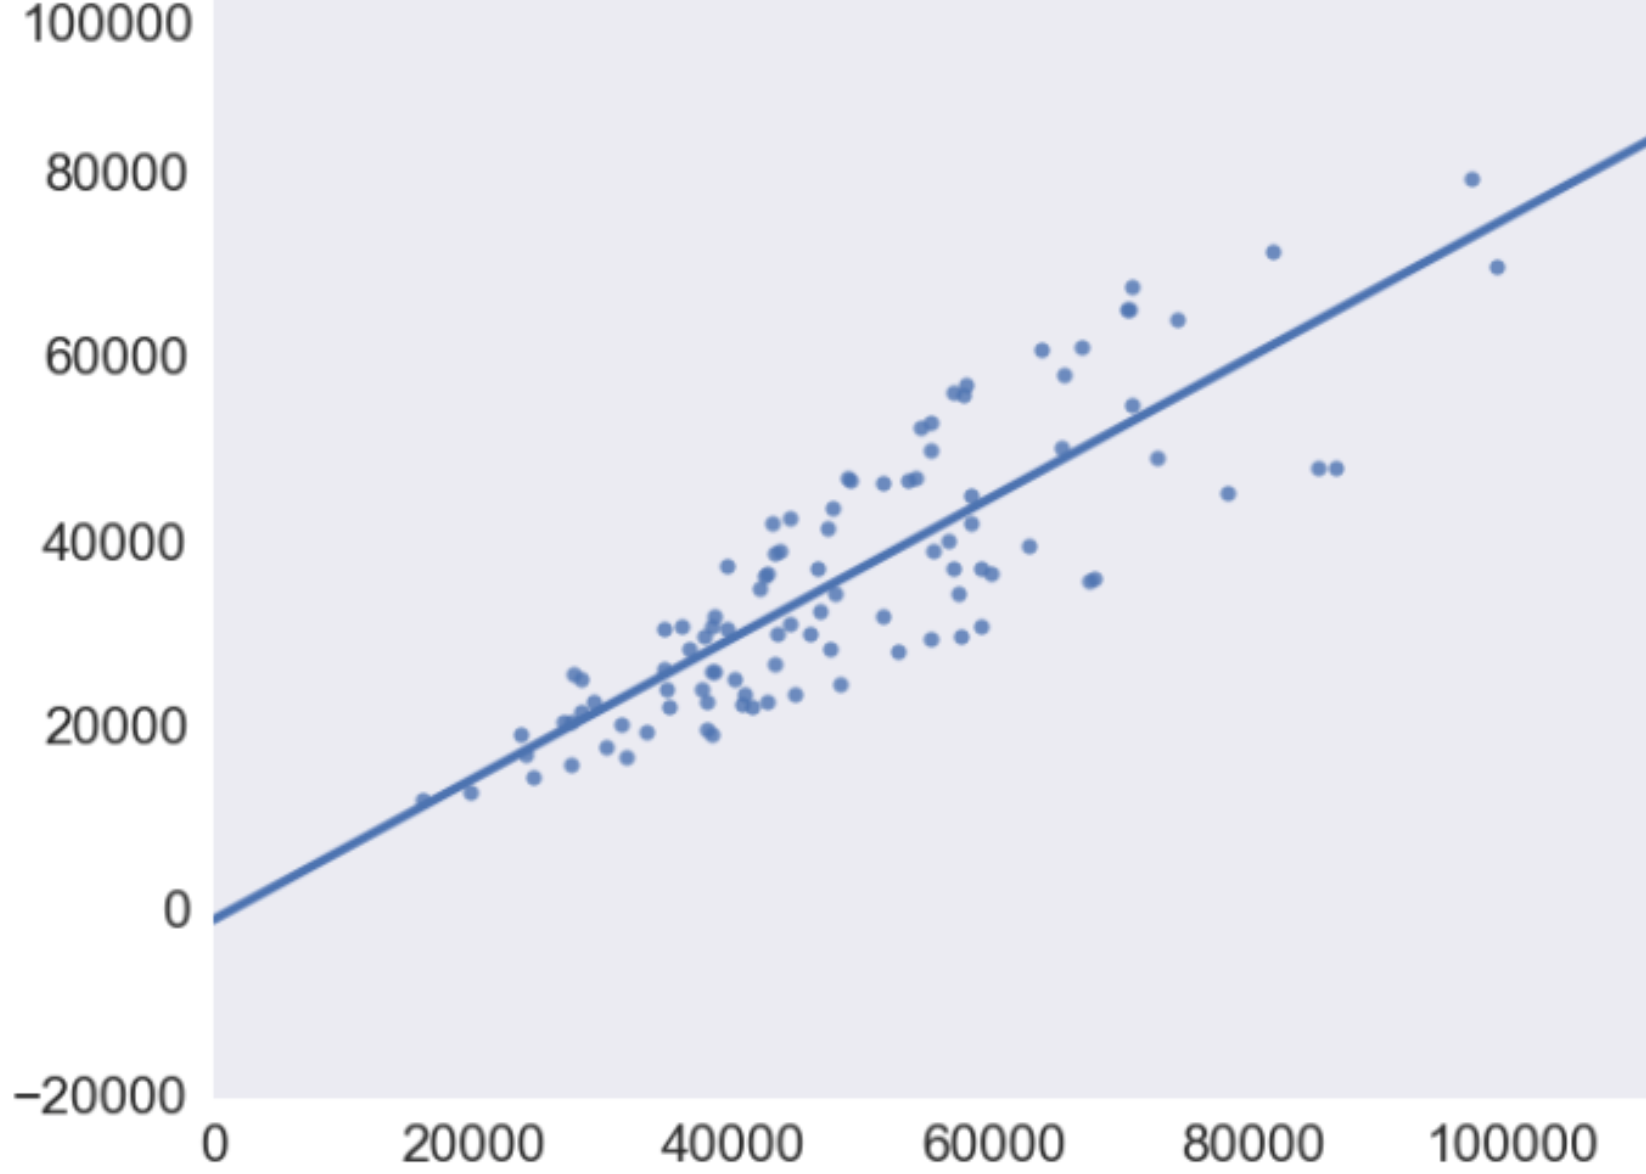
\includegraphics[width=2.1in]{stuff/log3.png}

\vspace{-1em}
\Large
\setlength{\leftmargini}{10pt}
\begin{itemize}
\item[]<2->
$$\text{Is this satisfactory}$$
$$\text{for predicting probability?}$$
$$\textcolor{red}{\onslide<3->{\text{How about this instead} \Longrightarrow}}$$
\end{itemize}

\end{column}
\begin{column}{.5\textwidth}

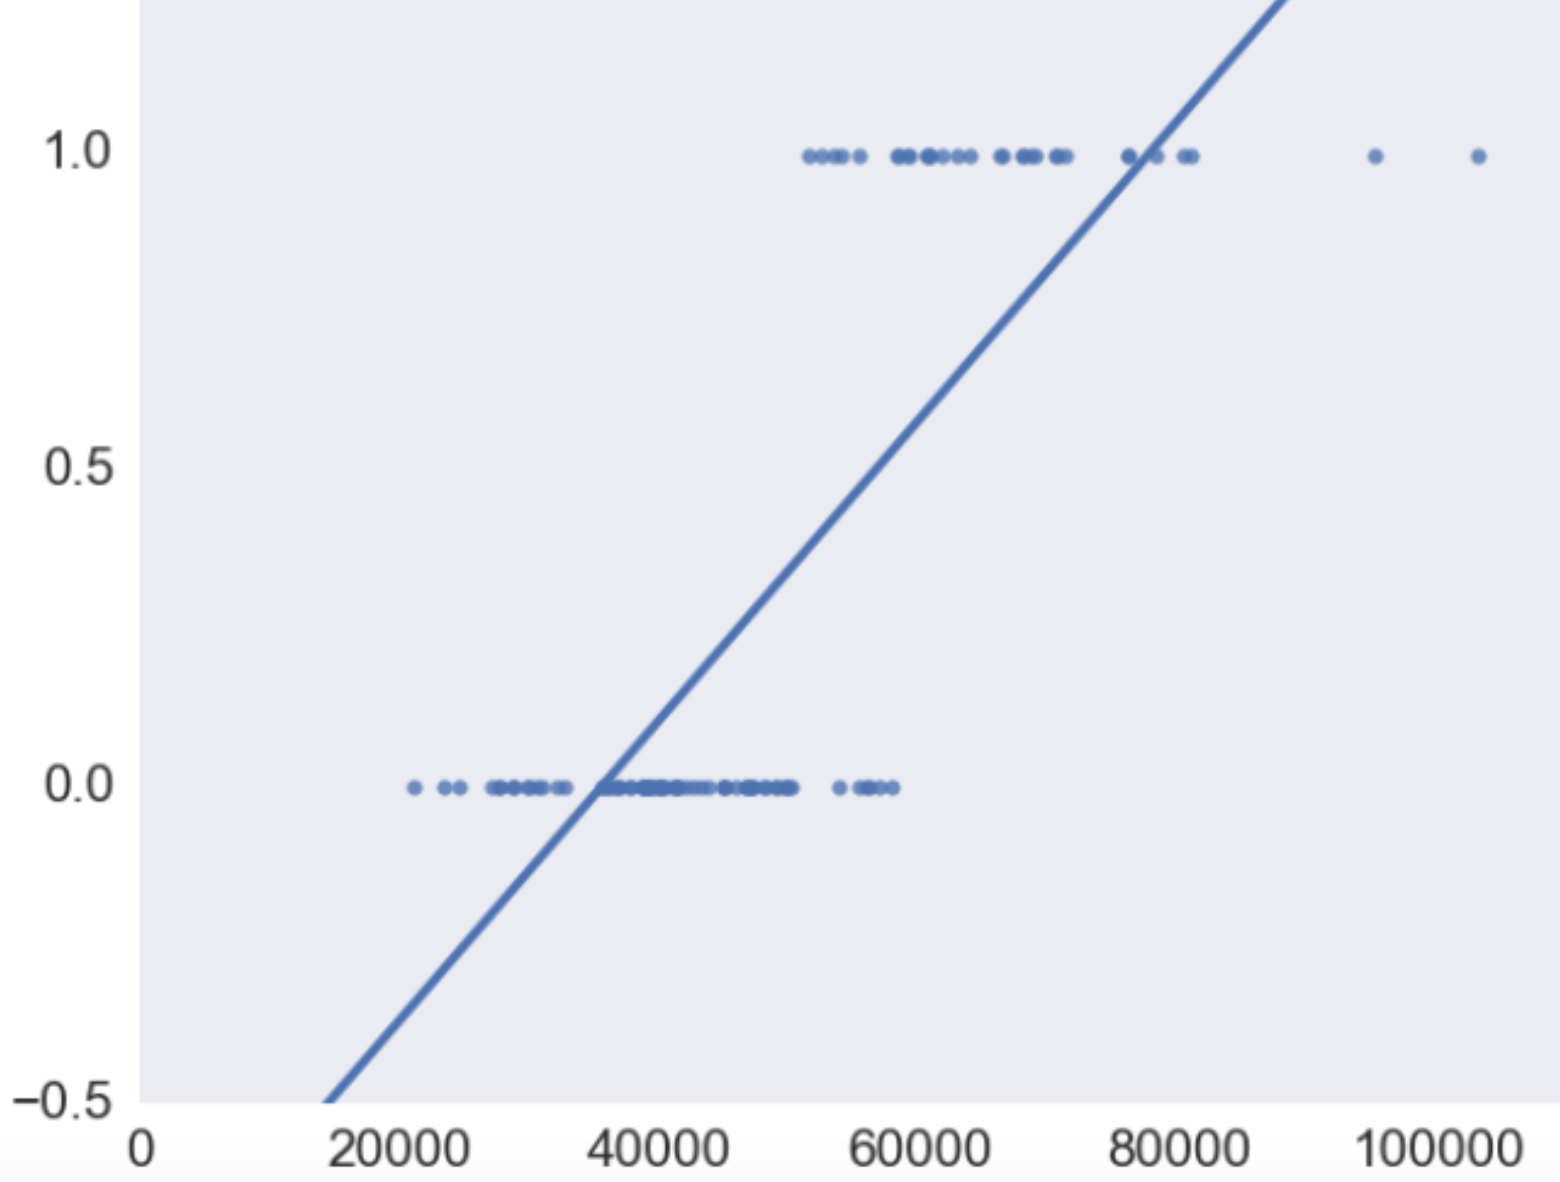
\includegraphics[width=2in]{stuff/log2.png}\\${}$

\vspace{-1em}
\setlength{\leftmargini}{0pt}
\begin{itemize}
\item[]<3->
\hspace{.4em}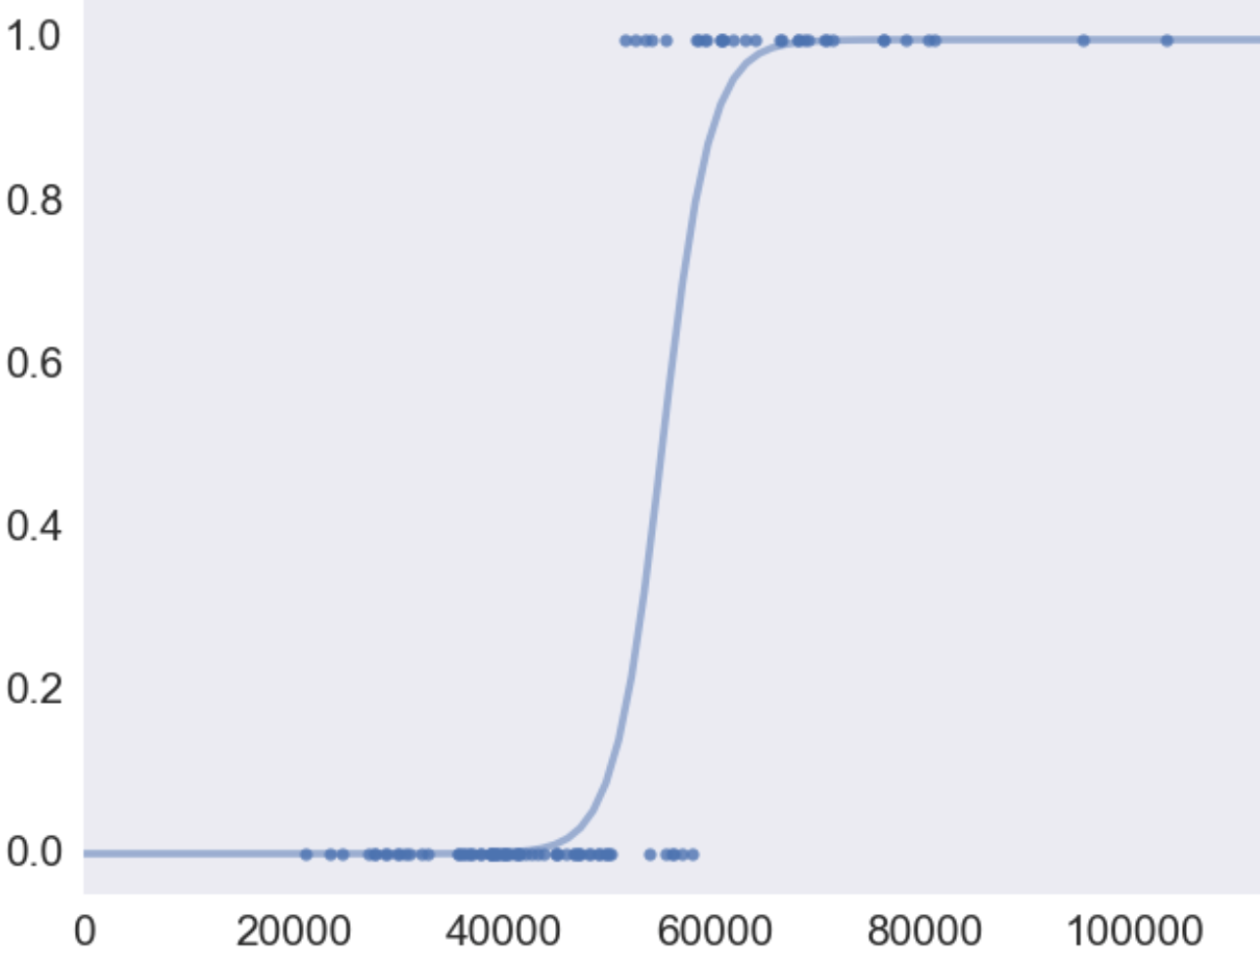
\includegraphics[width=1.925in]{stuff/log1.png}
\end{itemize}


\end{column}
\end{columns}
}




\frame
{
\frametitle{Link functions}

\begin{columns}
\begin{column}{.5\textwidth}
\begin{itemize}
\item The ``logit''  
$$g(p) = \log\left(\frac{p}{1-p}\right)$$
\item<2->  maps 
$$p \in {[}0,1{]} \mapsto Z \in \mathbb{R}$$
\item[]<3-> Probabilities are from 0 to 1 
\item[]<3-> But log odds go $-\infty$ to $\infty$! \\${}$
\item[]<4-> Don't be at odds with odds!
\end{itemize}
\end{column}
\begin{column}{.5\textwidth}
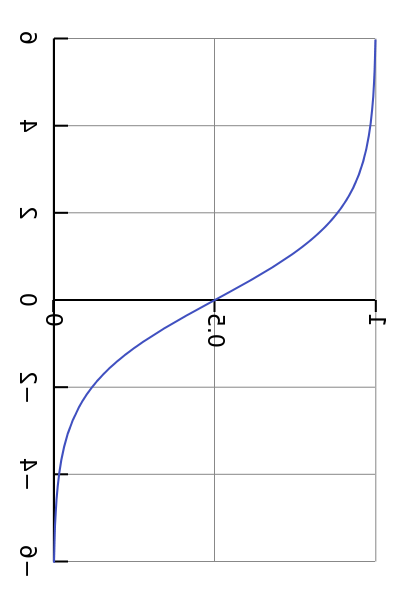
\includegraphics[width=2in]{stuff/Logistic-curve2.png}
\end{column}
\end{columns}
}



\frame
{
\frametitle{Logistic ``regression''}

\begin{itemize}
\item In Linear Model Regression, for \emph{real valued outcomes}, we used 
$$\hat Y_i \onslide<2->{= \text{E}\left[Y\right]} \onslide<2->{= Z = \beta_0 + \beta_1x_{1} + \cdots + \beta_mx_m}$$
\item<3-> 
For a \emph{binary} outcome $Y$, we instead define  
\begin{align*}
\hat Y_i = \text{Pr}\left(Y=1\right)  \onslide<4->{= \text{E}\left[Y\right]} \onslide<5->{= g^{-1}(Z)} \onslide<6->{&= \frac{\exp(Z)}{1+\exp(Z)}}
\end{align*}
\vspace{-5em}
\onslide<5>{\hspace{.7in}\textcolor{red}{because how else can Z stay between 0 and 1??}} 

\vspace{3em}
\onslide<6->{$\quad\quad\quad\quad\quad\quad\quad\quad\quad\quad\quad\quad\quad\quad\quad\quad\quad\;\;\; = \textcolor{red}{\frac{1}{1+\exp(-Z)}}$}

\end{itemize}

\vspace{1em}
$$\onslide<7->{\textcolor{black}{\text{So } g(p) = Z = \log\left(\frac{p}{1-p}\right) \textcolor{red}{ \in \mathbb R \;} \text{\textcolor{gray}{(which is called the logit function)}}}}$$
\vspace{-.5em}
$$\onslide<7->{\text{and } \underline{Z =  \beta_0 + \beta_1x_{1} + \cdots + \beta_mx_m \textcolor{red}{\; \in \mathbb R}\text{ models the log odds } }}$$ 

}

\frame
{
\frametitle{Linear model on log odds $\Longrightarrow$ transformed to probabilities}
 
\normalsize
\begin{figure}
\centering

Standard logistic (sigmoid) function
\Huge \onslide<3->{$\begin{array}{c}\hat Y\\\\\\\\\\ \; \end{array}$}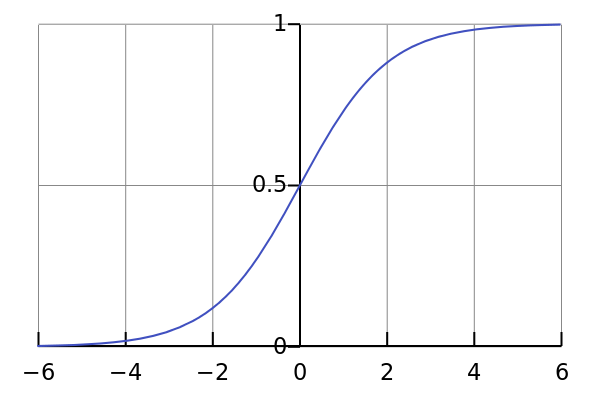
\includegraphics[width=3.25in]{stuff/Logistic-curve.png} \textcolor{white}{$\hat Y$} \normalsize

\vspace{-7em}
\onslide<2->{$Z =  \beta_0 + \beta_1x_{1} + \cdots + \beta_mx_m$\\${}$

\textcolor{gray}{(linear model on log odds)}}

\end{figure}
}


\frame
{
\frametitle{Logarithmic Scale}

\begin{itemize}
\item So
$$\text{Pr}(Y=1|x)  = \frac{1}{1 + e^{-(\beta_0 + \beta_1x_{1} + \cdots + \beta_nx_m )}}$$
\item<2-> And we can quickly see then that \\${}$

$\displaystyle \quad \frac{Pr(Y=1|x)}{Pr(Y=0|x)} \;\; = $
\vspace{-2.1em}
\item[]<3-> \hspace{9.2em}$\displaystyle \exp(\beta_0)\exp(\beta_1x_{1})\cdots\exp(\beta_mx_{m})$
\vspace{2.1em}
\end{itemize}

\begin{itemize}
\setlength\itemsep{1em}
\item<4-> So for a 1-unit increase in $x_{j}$\\
\onslide<5->{there is a  $\exp(\beta_j)$ multiplicative increase in \emph{the odds}}
\item<6-> I.e., \emph{the odds} are linear in $x$ on a multiplicative, i.e.,
 odds increase with $x$ on a \emph{logorithmic} scale with base $\exp(\beta_j)$
\item<7-> The $log$ odds $log\left( \frac{Pr(Y=1|x)}{Pr(Y=0|x)} \right)$ are on a linear scale
\hspace*{2in}$\textcolor{gray}{(\beta_0 + \beta_1x_{1} + \cdots + \beta_nx_m)}$
\end{itemize}
}

\frame
{
\frametitle{The Odds Ratio (OR)}

\begin{itemize}
\item Equivalently, $\exp(\beta_j)$ is the \emph{odds ratio (OR)} 
between 1-unit differences in $x_{j}$ (e.g., 0 versus 1) when other $x$'s are constant
$$ \text{exp}(\beta_j) =  \frac{Pr(Y=1|x_j+1,x_{-j})/Pr(Y=0|x_j+1,x_{-j})}{Pr(Y=1|x)/Pr(Y=0|x)}  $$
\textcolor{gray}{
since 
\begin{align*}
{} & \frac{Pr(Y=1|x_j+1,x_{-j})}{Pr(Y=0|x_j+1,x_{-j})} \\
= {} & \exp(\beta_0)\exp(\beta_1x_{1})\cdots\exp(\beta_j(x_{j}+1))\cdots\exp(\beta_mx_{m})\\
= {} & \exp(\beta_0)\exp(\beta_1x_{1})\cdots\exp(\beta_jx_{j})exp(\beta_j)\cdots\exp(\beta_mx_{m})\\
\text{and} {} & \\
{} & \frac{Pr(Y=1|x)}{Pr(Y=0|x)}  \\
= {} & \exp(\beta_0)\exp(\beta_1x_{1})\cdots\exp(\beta_jx_{j})\cdots\exp(\beta_mx_{m}) 
\end{align*}}
\vspace{-.75em}
\item<2-> So $\beta_j$ is the change in $log(OR)$ for one unit changes in $x_j$...
\item[]
\end{itemize}
}



\frame
{
\frametitle{Logistic Regression \emph{Likelihood} and \emph{Deviance}}

\begin{itemize}
\item Likelihood 
$$f(\textbf{Y}|{\boldsymbol \beta}, \textbf{x}) = \prod \left(\frac{1}{1+e^{-\textbf{x}_i^T \boldsymbol \beta }}\right)^{Y_i} \left(\frac{1}{1+e^{\textbf{x}_i^T\boldsymbol  \beta}}\right)^{1-Y_i} $$\\${}$
\item<2-> Deviance 
\begin{align*}
D_M ={} & -2\left( \text{log}f(\textbf{Y}|\hat {\boldsymbol \beta}, \textbf{x}) - \text{log}f(\textbf{Y}|\textbf{Y})\right) \\
\overset{\text{\tiny approx.}}{\sim} {} &  \chi^2_{n-p-1} \\ 
{}\\
n  = {} &  \text{sample size}\\
p  = {} & \text{number of coefficients in model }M\\
f(\textbf{Y}|\textbf{Y}) = {} &  \text{saturated model ($\textbf{Y}$ perfectly predicted)}
\end{align*}
\end{itemize}

}


\frame
{
\frametitle{More Deviance}

\begin{itemize}
\item In logistic regression \\
$D_M = -2\left( \text{log}f(\textbf{Y}|\hat {\boldsymbol \beta}, \textbf{x}) - \text{log}f(\textbf{Y}|\textbf{Y})\right) =$\\${}$
\item<2->[]
\hspace{-3em}$-2 \sum  Y_i log (p_i) + (1-Y_i) log (1-p_i) -  \textcolor{pink}{Y_i log (Y_i) - (1-Y_i) log (1-Y_i)}$ 
\vspace{-.5em}
$$\onslide<3->{\textcolor{gray}{\text{[show this]}}}\quad\quad\quad\quad\quad\quad\quad\quad\quad\quad\onslide<4->{\overset{\text{\tiny approx.}}{\sim} \chi^2_{n-p-1}}$$

\item<5-> In linear regression 
\begin{align*}
D_M = {}& \frac{RSS}{\sigma^2}\quad\quad\quad\quad\;\; \textcolor{gray}{\text{[show this]}} \\ %(n-k) \frac{1}{n-k} 
= {}& \frac{\sum (Y_i - \hat Y)^2}{\sigma^2} \textcolor{gray}{\;=  (n-p-1) \frac{s^2}{\sigma^2}} \overset{\text{\tiny approx.}}{\sim} \chi^2_{n-p-1}
\end{align*}

\item[]<6-> 
\hspace{-1em}$\textcolor{gray}{[\text{what are \emph{residuals}?}]} \quad \onslide<7->{\textcolor{gray}{[\text{what are \emph{``residuals''} in logistic regression?}]}}$

\end{itemize}
}



\frame
{
\frametitle{Fitting Logistic Regression}

\begin{itemize}
\item MLE
$$\hat {\boldsymbol \beta} = \underset{{\boldsymbol \beta}}{\text{argmax}} \prod \left(\frac{1}{1+e^{-\boldsymbol x^T \boldsymbol \beta}}\right)^{Y_i} \left(\frac{1}{1+e^{\boldsymbol x^T \boldsymbol \beta}}\right)^{1-Y_i}$$
$$ \textcolor{gray}{\Longleftrightarrow}$$
$$ \textcolor{gray}{\hat {\boldsymbol \beta} = \underset{ {\boldsymbol \beta}}{\text{argmin}} \; D_{{\boldsymbol \beta}} = \underset{ {\boldsymbol \beta}}{\text{argmax}} \left( \text{log}f(\textbf{Y}|\hat {\boldsymbol \beta}, \textbf{x}) - \text{log}f(\textbf{Y}|\textbf{Y})\right)}$$

\item<2->  \textcolor{Maroon}{Closed form solution not available (like with linear regression)}
\begin{itemize}
\item \textcolor{gray}{Optimization done via Newton-Rhapson or Gradient Decent}
\item \textcolor{gray}{Coefficient standard errors can also be numerically estimated!}
\end{itemize}

\item<3->  \textcolor{Maroon}{Convergence difficulties will be encountered if }
\begin{itemize}
\item \textcolor{gray}{too many features $(n/p < 10)$ or data is sparse/imbalanced }
\end{itemize}

\item<4->  \textcolor{Maroon}{Coefficient standard errors will be compromised when }
\begin{itemize}
\item \textcolor{gray}{predicted probabilities are only $\sim$1 or $\sim$0 (separated classes)}
\item \textcolor{gray}{There is covariate multicollinearity (as with linear regression)}
\end{itemize}

\item<5->  \textcolor{Maroon}{What if, for some $\lambda$,  we choose ${\boldsymbol \beta}$ to minimize}
$$ -\prod \left(\frac{1}{1+e^{-\textbf{x}^T_i {\boldsymbol \beta}}}\right)^{Y_i} \left(\frac{1}{1+e^{\textbf{x}^T_i {\boldsymbol \beta}}}\right)^{1-Y_i} + \lambda ||{\boldsymbol \beta}||^2? $$

\end{itemize}
}




\frame
{
\frametitle{Fitting Logistic Regression}

\begin{itemize}
\item MLE
$$\hat {\boldsymbol \beta} = \underset{{\boldsymbol \beta}}{\text{argmax}} \prod \left(\frac{1}{1+e^{-\boldsymbol x^T \boldsymbol \beta}}\right)^{Y_i} \left(\frac{1}{1+e^{\boldsymbol x^T \boldsymbol \beta}}\right)^{1-Y_i}$$
$$ \textcolor{gray}{\Longleftrightarrow}$$
$$ \textcolor{gray}{\hat {\boldsymbol \beta} = \underset{{\boldsymbol \beta}}{\text{argmin}} \; D_{\boldsymbol \beta} = \underset{{\boldsymbol \beta}}{\text{argmax}} \left( \text{log}f(\textbf{Y}|\hat {\boldsymbol \beta}, \textbf{x}) - \text{log}f(\textbf{Y}|\textbf{Y})\right)}$$


\item \textcolor{Maroon}{Closed form solution not available (like with linear regression)}
\begin{itemize}
\item  \textcolor{gray}{Optimization done via Newton-Rhapson or Gradient Decent}
\item \textcolor{gray}{Coefficient standard errors can also be numerically estimated!}
\end{itemize}

\item \textcolor{Maroon}{Convergence difficulties will be encountered if} 
\begin{itemize}
\item \textcolor{gray}{too many features $(n/p < 10)$ or data is sparse/imbalanced} 
\end{itemize}

\item \textcolor{Maroon}{Coefficient standard errors will be compromised when} 
\begin{itemize}
\item \textcolor{gray}{predicted probabilities are only $\sim$1 or $\sim$0 (separated classes)}
\item \textcolor{gray}{There is covariate multicollinearity (as with linear regression)}
\end{itemize}

\item  \textcolor{Maroon}{What if, for some $\lambda$,  we choose $\boldsymbol \beta$ to minimize} 
$$ -\prod \left(\frac{1}{1+e^{-\textbf{x}^T_i{\boldsymbol \beta}}}\right)^{Y_i} \left(\frac{1}{1+e^{\textbf{x}^T_i{\boldsymbol \beta}}}\right)^{1-Y_i} + \lambda | {\boldsymbol \beta}|_1? \;\;$$

\end{itemize}


% minimize AIC/BIC (you see that/why?)
% when doing regression talk about types categorical, continuous, indicator

% odds ratio: "this many times more likely"

% uses -- see uses slides

% roc -- why is that worse than random guessing?
}



\frame
{
\frametitle{Pseudo $R^2$}

\begin{itemize}
\item McFadden's \emph{pseudo} $R^2 = 1 - D_M/D_0$
\item[]<2-> Proportion of deviance explained
\item[]
\item<3->  \textcolor{gray}{Compare to linear model $R^2 = 1 - RSS/TSS$}
\item[]<3->  \textcolor{gray}{Proportion of variance explained}
\item[]
\item<4->
\url{http://www.ats.ucla.edu/stat/mult_pkg/faq/general/Psuedo_RSquareds.htm}
\end{itemize}
}

\frame
{
\frametitle{Model Comparison}

\begin{itemize}
\item[] \textcolor{gray}{Remember, $D_M = -2(log f(\textbf{Y}|\hat \theta_M) - log f(\textbf{Y}|\textbf{Y}))$, so}
\item<2-> comparison of \textcolor{gray}{(\emph{reduced} and \emph{full})} models can be done using
$$D_R - D_F = -2\left( \text{log}f(Y|\hat \theta^R) - \text{log}f(Y|\hat \theta^F)\right) \overset{\text{\tiny approx.}}{\sim} \chi^2_k$$ 
where model $R$ is nested in model $F$ with $k$ fewer parameters
\item[] 
\item<3->
For \emph{non-nested} models, compare
\begin{align*}
AIC :{}& -2 \text{log}f(Y|\hat \theta) + 2k \\
BIC :{}& -2 \text{log}f(Y|\hat \theta) + k \text{log}(n) 
\end{align*}
\item[]<4-> \huge $\quad$How else could you compare\\$\quad$nested or non-nested models?
\end{itemize}
}

\frame
{
\frametitle{Uses for logistic regression?}

\Large 
\begin{itemize}
\item<2-> Predict probabilities
\item<3-> Classify outcomes (based on probabilities)
\item<4-> Identify feature associations with class labels
\item[]
\item<5-> \textcolor{gray}{Balancing observational comparison groups on \emph{propensity scores} Pr($T|x$) which controls bias from group covariate composition differences}
% [talk a bit about experimental design?] 

\end{itemize}
}


\frame
{
\frametitle{Confusion Matrix (and questions)}

\begin{figure}
\centering
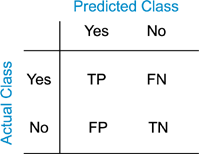
\includegraphics[width=2.5in]{stuff/confusionmatrix.png}
\end{figure}

\begin{itemize}
\item[]<2-> Which cells are Type I and Type II error?
\item[]<3-> What is the power of a test? \onslide<4->{Pr(Reject $H_0$ $|$ $H_A$ True)} 
\item[]<5-> And the $\alpha$-significance level? \onslide<6->{Pr(Reject $H_0$ $|$ $H_0$ True)}

\end{itemize}

}


\frame
{
\frametitle{Sensitivity \& Specificity}

\begin{itemize}
\item Sensitivity:  \% of ``true $H_A$''  tests \underline{correctly called} $\left(\frac{\#TP}{\#TP+\#FN}\right)$
\begin{itemize}
\item[] \textcolor{gray}{``How \textbf{sensitive} are we to variations from $H_0$?''}
\item[]
\item<2-> \textcolor{Maroon}{Also called \emph{True Positive Rate}}
\item<2-> \textcolor{Maroon}{Also called \emph{Recall}}
\end{itemize}
\item[]
\item<3-> Specificity:  \% of ``true $H_0$''  tests \underline{correctly called} $\left(\frac{\#TN}{\#TN + \#FP}\right)$
\begin{itemize}
\item[]<3-> \textcolor{gray}{``How \textbf{specific} must evidence against $H_0$ be?''}
\item[]
\item<4-> \textcolor{Maroon}{Also called \emph{True Negative Rate}}
\item<4-> \textcolor{Maroon}{The ``1 minus'' related \emph{False Positive Rate} is $\left(\frac{\#FP}{\#TN+\#FP}\right)$}
\end{itemize}
\item[]
\item<5-> Test \emph{power}, $1-\beta = $  Pr(Reject $H_0$ $|$ $H_A$ True), \textbf{${\boldsymbol I}\hspace{-.1em}{\boldsymbol S}$ Sensitivity} 
\item<5-> $\alpha$-significance level, Pr(Reject $H_0$ $|$ $H_0$ True), \textbf{${\boldsymbol I}\hspace{-.1em}{\boldsymbol S}$ 1-Specificity } 
\item<6-> I.e, Type I \& II error rates \textbf{are 1-Specificity \& 1-Sensitivity}
\end{itemize}
}



\frame
{
\frametitle{ROC/AUC}


\begin{columns}
\begin{column}{.05\textwidth}
\end{column}
\begin{column}{.1\textwidth}
\onslide<2->{\hspace*{0in}\rotatebox{90}{$\quad\quad$\emph{Power} $ = 1 - \beta$}}
\end{column}
\hspace*{-1.5in}
\begin{column}{.9\textwidth}
\begin{figure}
\centering
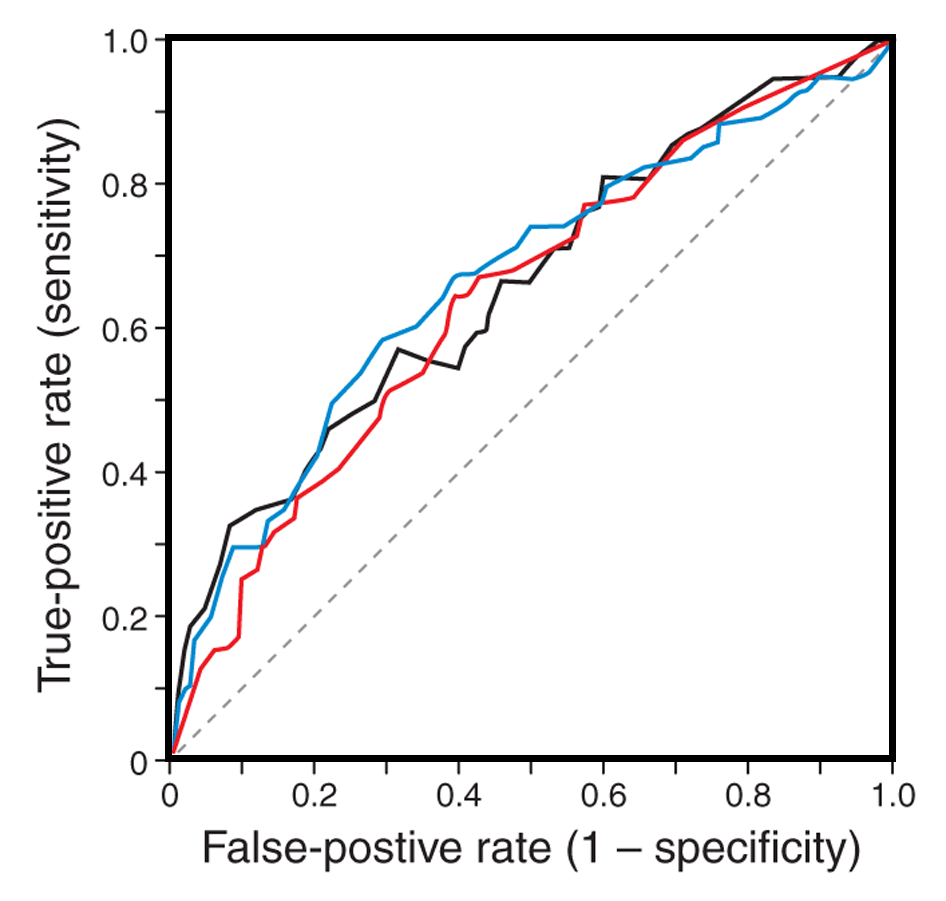
\includegraphics[width=2.5in]{stuff/roc.png}\\
\vspace{-.5em}
\onslide<2->{$\quad\quad\alpha$\\${}$\\}
\end{figure}
\end{column}
\end{columns}

\onslide<3->{
\url{https://www.youtube.com/watch?v=JAQC59ArFJw}
\url{https://www.youtube.com/watch?v=bhvvxNUbIpo}}
}



\frame
{
\frametitle{Other BIGGIES: \emph{precision, FDR, and accuracy}}

\vspace{-2.5em}

\hspace*{-1em}\begin{columns}
\begin{column}{1.1\textwidth}

\small

\begin{itemize}
\item Precision:  \% \textbf{positives} \underline{called \textbf{correctly}} $\left(\frac{\#TP}{\#TP+\#FP}\right)$
\item[]
\begin{itemize}
\item<2->[] \textcolor{gray}{``How ${\boldsymbol P}$\emph{recise} are we in our `${\boldsymbol P}$\emph{ositives}' (when we reject $H_0$)?''}
\item[]
\item<3-> \textcolor{Maroon}{Also called \emph{Positive Predicted Value}}
\end{itemize}
\item[]
\item<4-> False Discovery Rate (FDR):  \% \textbf{positives} \underline{called \textbf{incorrectly}} $\left(\frac{\#FP}{\#TP+\#FP}\right)$
\item[]
\begin{itemize}
\item<5->[] \textcolor{gray}{``What's the error rate in our significant tests?''}
\item[]
\item<6-> \textcolor{Maroon}{\emph{VERY} useful concept of multiple testing contexts}
\item[]<6-> \textcolor{Maroon}{a.k.a. for a \emph{multiplicity adjustment} (where it's called a \emph{q-value})}
\end{itemize}
\item[]
\item<7-> Accuracy:  \% of tests we \underline{we correctly call} $\left(\frac{\#TP+\#TN}{\#Total}\right)$
\item[]
\begin{itemize}
\item<8->[] \textcolor{gray}{``Do we call hypotheses \textbf{accurately}?''}
\end{itemize}
\end{itemize}

\end{column}
\end{columns}

}



\frame
{
\frametitle{And just a one or two more...}

\vspace{2em}

\hspace*{-.25in}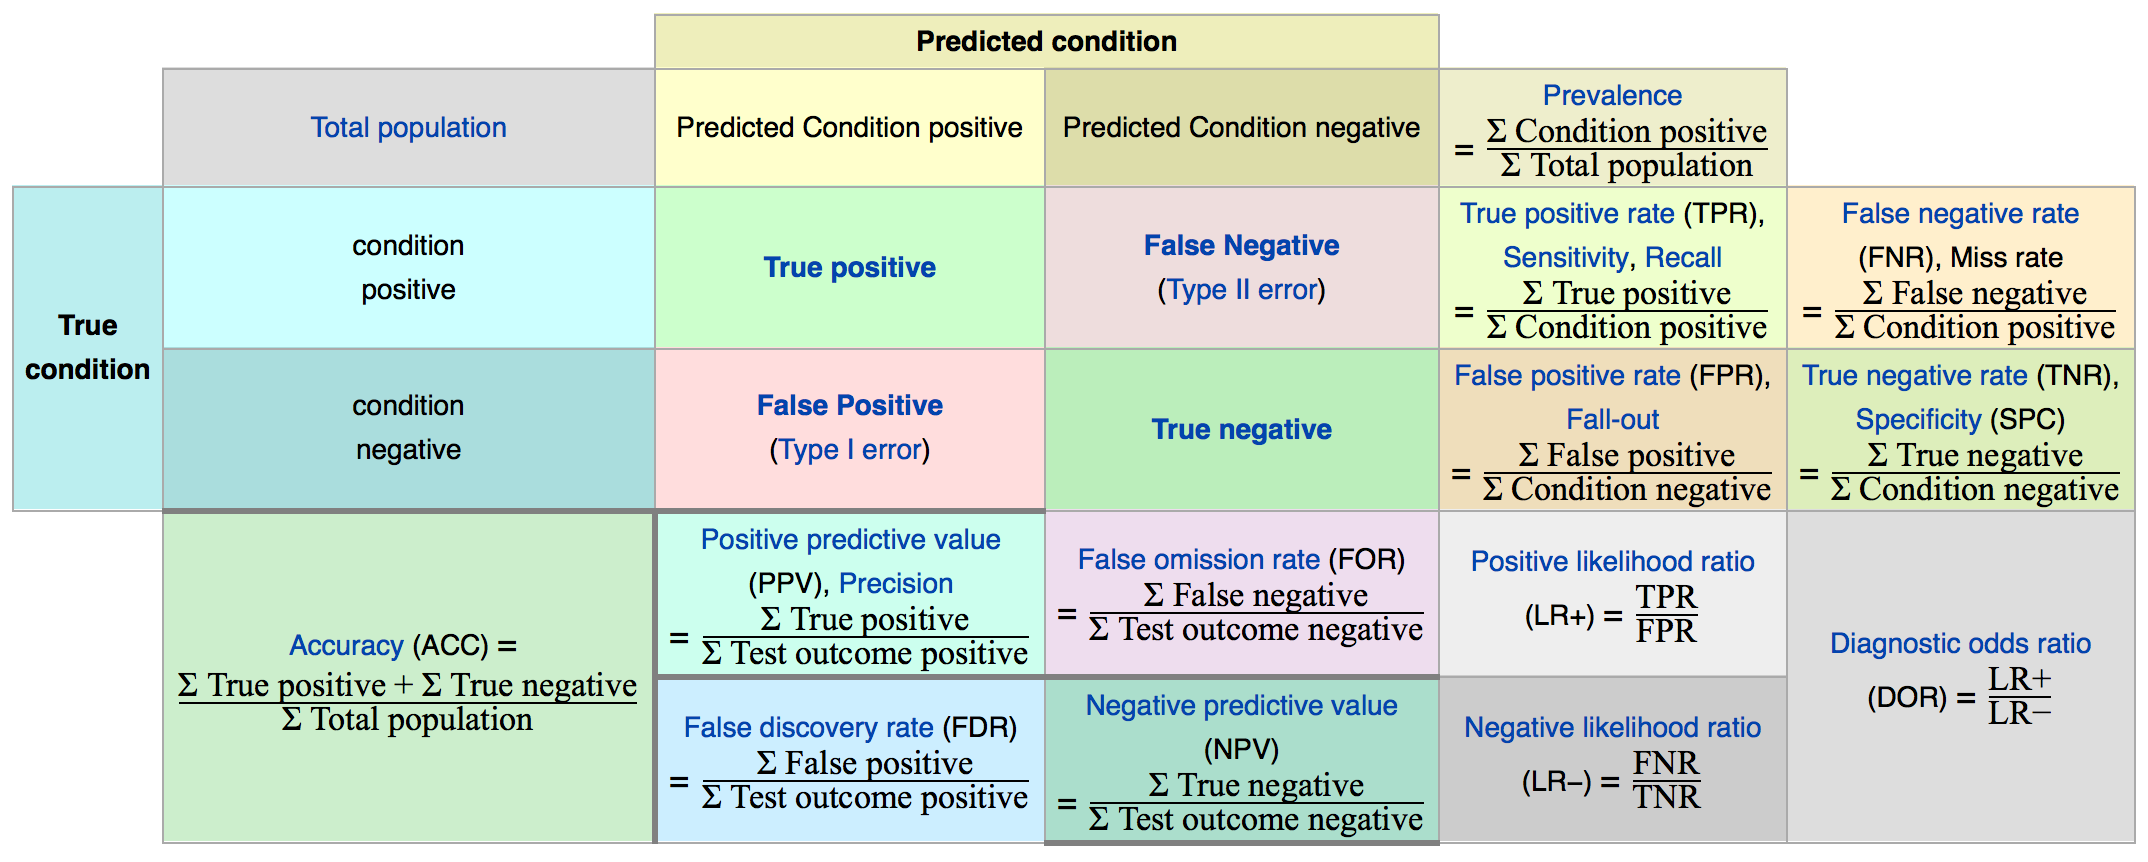
\includegraphics[width=4.75in]{stuff/terminology.png}

\begin{figure}
\centering
Thanks, Wiki! 

\footnotesize
\textcolor{gray}{(You're the besht!)}
\end{figure}

}







\end{document}


